\documentclass[a4paper,11pt]{article}
\usepackage{graphicx,msc,alltt,float,geometry,tikz,pgf-umlcd,listings,alloy,hyperref}
\setcounter{tocdepth}{2}

\geometry{
	includeheadfoot,
	margin=2.54cm
}

\lstset{ %
  language=alloy,                % the language of the code
  basicstyle=\footnotesize,       % the size of the fonts that are used for the code
  numbers=left,                   % where to put the line-numbers
  numberstyle=\tiny\color{gray},  % the style that is used for the line-numbers
  stepnumber=1,                   % the step between two line-numbers. If it's 1, each line 
                                  % will be numbered
  numbersep=5pt,                  % how far the line-numbers are from the code
}

\begin{document}
	\begin{titlepage}
	\begin{center}

		{\Huge 2IW05 Software Specification\\ Project}\\[0.5cm]
		{\huge Deliverable 1}\\
		\rule{\linewidth}{0.5mm}\\[0.5cm]


		{\Large
		Tim van Dalen\\
		Carl van Dueren den Hollander\\
		Bart Koopmans\\[1cm]
		}

		{\large
		Department of Computer Science\\
		Technical University Eindhoven\\[1cm]
		}

		\begin{abstract}

This document gives a basic formal specification for the 2IW05 'Doodle' project. It contains use-cases for modelling a system, an analysis model for this system and a design model that provides a design for the system.

We will also state some possible improvements over this basic system.

\end{abstract}

		\vfill

		{\large \today}
	\end{center}
\end{titlepage}

	\tableofcontents
	\newpage

	\section{Introduction}
	This document presents a formal specification for the 'Doodle' meeting website for the 2012 fall 2IW05 software specification course.

We will follow a normal iterative approach (with only two iterations for two deliverables) where we will first extract use cases from the informal specification and use them to analyse the informal specification. Then we will use this analysis to form a system design.

	\newpage
	
	\section{Use cases}
	This section describes the use cases of the system.

\subsubsection{Create meeting schedule}

\begin{description}
	\item[Pre-condition:] User is registered and logged in
	\item[Trigger:] User clicks 'Schedule new event' link
	\item[Guarantee:] A new event is created
	\item[Scenarios]\textbf{:}\\
				\begin{description}
					\item[Main scenarios]\textbf{:}\\
								\begin{enumerate}
									\item The user enters his/her name, the event name and an event description
									\item The user enters some date/time options
									\item The user enters email addresses for attendees and a custom message
									\item The user specifies whether or not the poll should be 'hidden' and voting limitations
									\item The user submits the event to the system by openeing the poll
								\end{enumerate}
					\item[Alternatives]\textbf{:}\\
								\begin{itemize}
									\item 2.1 One or more date/time pairs are not valid, the system shows an error message and the user is back at the start of step 2, with all fields already filled in, except for the rrorous ones.
								\end{itemize}
				\end{description}
\end{description}


\subsubsection{Respond to a meeting invitation}

\begin{description}
	\item[Pre-condition:] User has received an invitation email and the meeting poll is open
	\item[Trigger:] User clicks the link in the invitation email
	\item[Guarantee:] The user voted on possible dates
	\item[Scenarios]\textbf{:}\\
				\begin{description}
					\item[Main scenarios]\textbf{:}\\
								\begin{enumerate}
									\item The user confirms that he or she would like to attend the event
									\item The user votes on date/time options
									\item The system sends a notification email to the organizer
									\item The user is able to see the votes of other invitees
								\end{enumerate}
					\item[Alternatives]\textbf{:}\\
								\begin{itemize}
									%TODO: Not sure if an alternative is really the way to go. I used to have a seperate use case for accepting and declining, but that seemed a bit superfluous.
									\item 1.1 If the user doesn't want to participate in the event, he or she declines the invitation.	
									\item 2.1 If the organizer made any voting restrictions, such as enabling users to only vote once or limiting the number of invitees that can vote on a certain date/time, these are enforced.
									\item 4.1 If the poll was marked 'hidden' by the organizer, the results are not shown
								\end{itemize}
				\end{description}
\end{description}

\subsubsection{Edit a meeting response}

\begin{description}
	\item[Pre-condition:] User has responded to a meeting invitation and the meeting poll is open
	\item[Trigger:] User clicks the link in the invitation email
	\item[Guarantee:] The users answer/votes might have been changed.
	\item[Scenarios]\textbf{:}\\
				\begin{description}
					\item[Main scenarios]\textbf{:}\\
								\begin{enumerate}
									\item The user confirms that he/she would still like to attend the event
									\item The user votes on date/time options
									\item The system sends a notification email to the organizer
									\item The user is able to see the votes of other invitees
								\end{enumerate}
					\item[Alternatives]\textbf{:}\\
								\begin{itemize}
									\item 1.1 If the user doesn't want to participate anymore, he or she can decide to decline the invitation.
									\item 4.1 If the poll was marked 'hidden' by the organizer, the results are not shown
								\end{itemize}
				\end{description}
\end{description}

\subsubsection{Administrate an event}

\begin{description}
	\item[Pre-condition:] The user is the organizer for this event
	\item[Trigger:] User clicks the link to administrate the event
	\item[Guarantee:] Settings for the event might have changed
	\item[Scenarios]\textbf{:}\\
				\begin{description}
					\item[Main scenarios]\textbf{:}\\
								\begin{enumerate}
									\item The user is presented with an overview of the event.
									\item The user chooses to delete the event, edit the general settings, change the date/time options or view event logs.
								\end{enumerate}
				\end{description}
\end{description}

\subsubsection{Close an event}

\begin{description}
	\item[Pre-condition:] The user is the organizer for this event
	\item[Trigger:] User clicks the link to administrate the event and then clicks the delete button
	\item[Guarantee:] The event is closed
	\item[Scenarios]\textbf{:}\\
				\begin{description}
					\item[Main scenarios]\textbf{:}\\
								\begin{enumerate}
									\item The user is presented with a modal dialog asking them if they are sure. The user clicks 'yes'.
									\item The user selects the final date/time based on the poll results.
									\item Optionally, the user enters a closing message for the event
									\item An email containing the optional message and the final date/time is sent to each invitee that confirmed.
									\item The event is closed.
								\end{enumerate}
					\item[Alternatives]\textbf{:}\\
								\begin{itemize}
									\item 1.1 If the user clicks 'no', the closing is cancelled.
								\end{itemize}

				\end{description}
\end{description}


	\newpage
	
	\section{Analysis}
	This section aims to give a first analysis of the system.

\subsection{High-level entities}
	Figure~\ref{fig:analysis-model} identifies the high-level entities in the system.
	
	\begin{figure}[H]
		\centering
		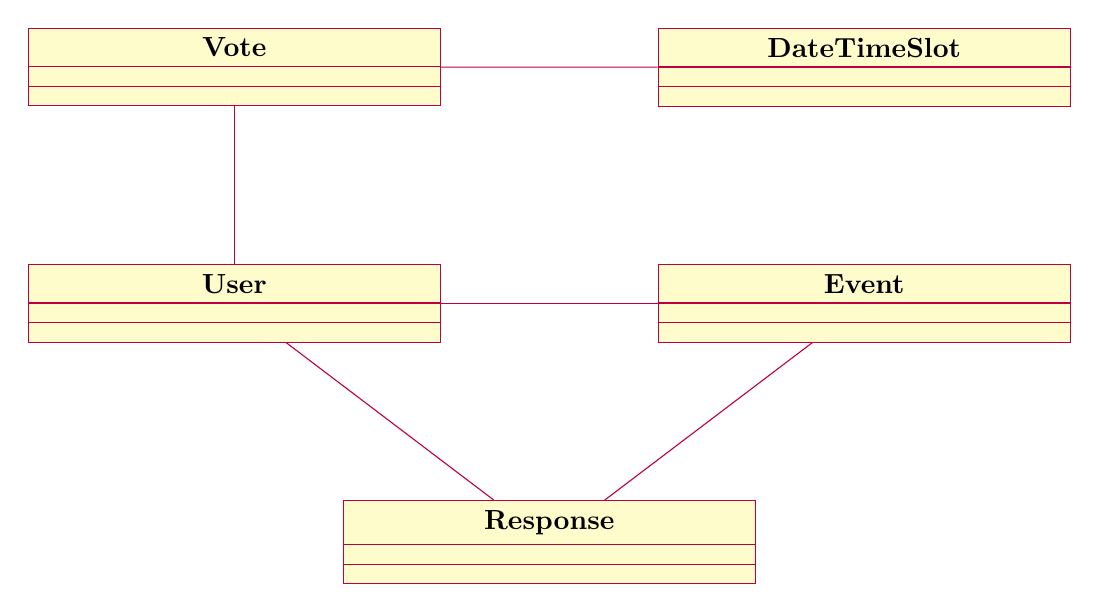
\begin{tikzpicture}
			\begin{class}{User}{0,3}
			\end{class}
		
			\begin{class}{Vote}{0,6}
			\end{class}

			\begin{class}{DateTimeSlot}{8,6}
			\end{class}


			\begin{class}{Event}{8,3}
			\end{class}

			\begin{class}{Response}{4,0}
			\end{class}

			\association{Response}{}{}{User}{}{}
			\association{Response}{}{}{Event}{}{}
			\association{DateTimeSlot}{}{}{Vote}{}{}
			\association{Vote}{}{}{User}{}{}
			\association{User}{}{}{Event}{}{}
		\end{tikzpicture}
		\caption{High-level entities in the system}
		\label{fig:analysis-model}
	\end{figure}
	
\subsection{System level sequence diagram}
	%Note: These should be for each use case, with System one entity and entities for the actors
%\begin{figure}[H]
%%\centering
%%\begin{msc}{Use case 1}
%%%\declinst{usr}{User}{}
%%%\declinst{sys}{System}{}
%%%
%%%\mess{Message}{usr}{sys}
%%\end{msc}
%%\caption{One}
%%\label{smsc:one}
%\end{figure}

	\newpage
	
	\section{Design model}
	\subsection{Class diagram}
	\begin{figure}[H]
		\centering
		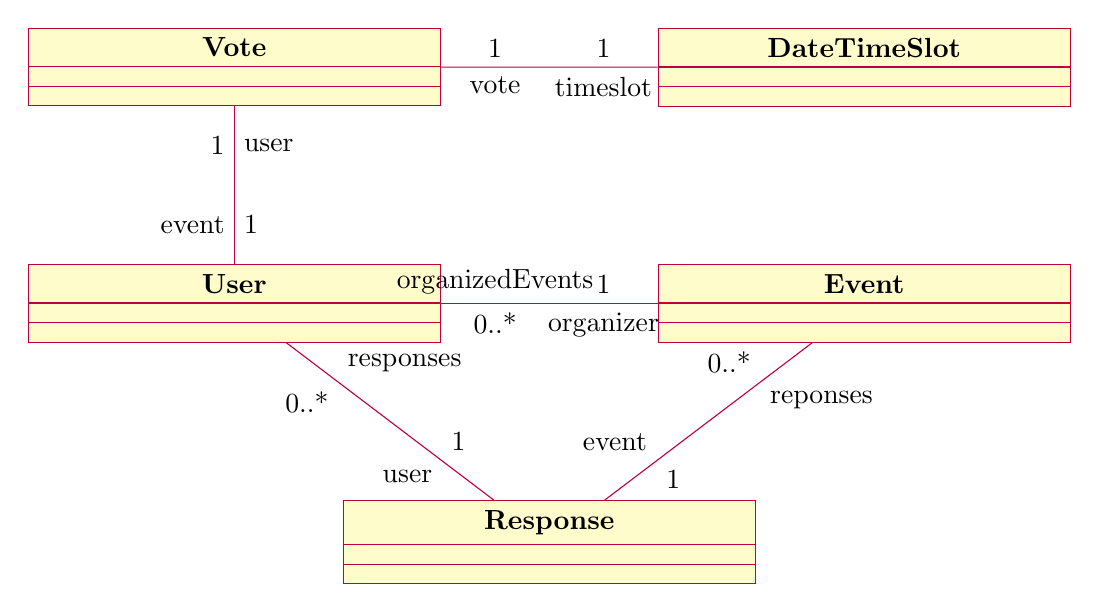
\begin{tikzpicture}
			\begin{class}{User}{0,3}
			\end{class}
		
			\begin{class}{Vote}{0,6}
			\end{class}

			\begin{class}{DateTimeSlot}{8,6}
			\end{class}


			\begin{class}{Event}{8,3}
			\end{class}

			\begin{class}{Response}{4,0}
			\end{class}

			\association{Response}{user}{1}{User}{0..*}{responses}
			\association{Response}{event}{1}{Event}{0..*}{reponses}
			\association{DateTimeSlot}{timeslot}{1}{Vote}{vote}{1}
			\association{Vote}{user}{1}{User}{1}{event}
			\association{User}{organizedEvents}{0..*}{Event}{1}{organizer}
		\end{tikzpicture}
		\caption{High-level entities in the system}
		\label{fig:class-diagram}
	\end{figure}

\subsection{Message Sequence Diagrams}
	\subsubsection{One}
		This MSC describes...
%%\begin{figure}[H]
%%%\centering
%%%\begin{msc}{One}
%%%%\declinst{comp}{Component 1}{}
%%%%\declinst{compt}{Component 2}{}
%%%
%%%%\mess{Message}{comp}{compt}
%%%\end{msc}
%%%\caption{One}
%%%\label{msc:one}
%%\end{figure}

	\newpage
	
	\section{Formal Specification}
	This section gives a formal specification of our system. Our class diagram has some redundant links in it, which made the specification much harder. When we figured out why some of our predicates were invalid, we didn't have time to change the model anymore, so we tried deep comparing instead of normal comparing.

An example of this is the \texttt{addResponse} predicate. We wanted to specify that the new set of responses was the old set of responses unioned with a singleton containing the new response, but because of the links in Response, User and Event, this was not possible.

\subsection{Sigs}
	\subsubsection{Core module}
		This is our core module. Because of some of the predicates, all sigs have to be in here, except for DateTimeSlot.
	
		\lstinputlisting{alloy/Core.als}
	
	\subsubsection{DateTimeSlot}
	
		\lstinputlisting{alloy/DateTimeSlot.als}
	
\subsection{Facts}
	All facts about the core are in one module, factsCore.
	
	\lstinputlisting{alloy/factsCore.als}
	
\subsection{Preds}
	\subsection{Show the core}
		A trivial predicate to show everything.
		
		\lstinputlisting{alloy/predShowCore.als}
		
	\subsection{Event}
		Some predicates for the Event sig.
		
		\lstinputlisting{alloy/predsEvent.als}
		
	\subsection{Poll}
		Some predicates for the Poll sig.
		
		\lstinputlisting{alloy/predsPoll.als}
		
\subsection{Trace}
	The following images give a trace of our specification.
	
	\subsubsection{Core}
		\inputgraphics[width=\linewidth]{alloy/trace/show}
		
	\subsection{Open Poll}
		\inputgraphics[width=\linewidth]{alloy/trace/poll1}
		
		\inputgraphics[width=\linewidth]{alloy/trace/poll2}
		
	\subsection{Adding vote}
		\inputgraphics[width=\linewidth]{alloy/trace/vote1}
		
		\inputgraphics[width=\linewidth]{alloy/trace/vote2}
	
\subsection{Get the specification}
	To download this complete set of files, you can clone our git repository at \texttt{git://github.com/timvdalen/2IW05-project.git}. You can also browse the code online at \url{https://github.com/timvdalen/2IW05-project/tree/master/alloy}.
	\newpage
	
\end{document}
